\documentclass[tikz,border=3pt]{standalone}
\usepackage[utf8]{inputenc}
\usepackage[T1]{fontenc}
\usepackage{lmodern}
\renewcommand{\familydefault}{\sfdefault}
\usepackage{sansmath}\sansmath
\usepackage{chemfig}
\usepackage{pgfplots}\pgfplotsset{compat=1.18,/pgf/number format/use comma,/pgf/number format/1000 sep={.}}
\usetikzlibrary{arrows.meta,calc,positioning,decorations.pathmorphing,patterns}
% paleta del sitio
\definecolor{nar}{HTML}{E8680C}\definecolor{narc}{HTML}{FFB35C}\definecolor{hielo}{HTML}{FFF3E8}
\definecolor{tinta}{HTML}{1D1D1F}\definecolor{gris}{HTML}{6E6E73}\definecolor{lila}{HTML}{7C5CF0}
\definecolor{azul}{HTML}{2F6FD6}\definecolor{menta}{HTML}{17A673}\definecolor{coral}{HTML}{E8342A}
\begin{document}
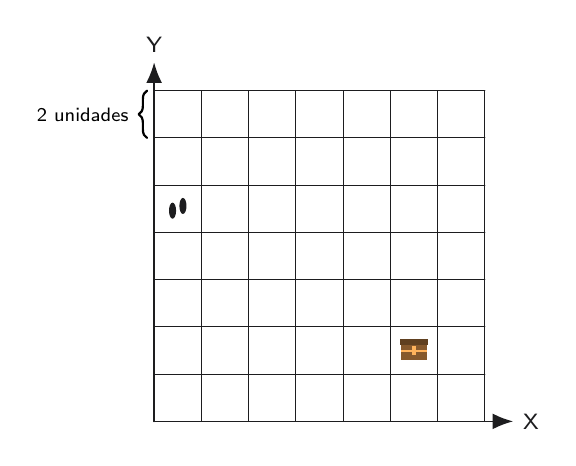
\begin{tikzpicture}[font=\small,x=0.6cm,y=0.6cm,line cap=round,line join=round,step={(1,1)}]
\draw[tinta,thin] (0,0) grid (7,7);
\draw[-{Latex[length=2.6mm,width=2mm]},tinta,semithick] (0,0)--(7.6,0) node[right,font=\footnotesize] {X};
\draw[-{Latex[length=2.6mm,width=2mm]},tinta,semithick] (0,0)--(0,7.6) node[above,font=\footnotesize] {Y};
\draw[decorate,decoration={brace,amplitude=3pt},thick] (-0.15,6)--(-0.15,7) node[midway,left=3pt,font=\scriptsize] {2 unidades};
\fill[tinta] (0.39,4.46) ellipse (0.075 and 0.17);\fill[tinta] (0.61,4.56) ellipse (0.075 and 0.17);
\fill[brown!70!black] (5.22,1.3) rectangle (5.78,1.62); \fill[narc] (5.22,1.47) rectangle (5.78,1.52);
\fill[brown!50!black] (5.2,1.62) rectangle (5.8,1.75); \fill[narc] (5.46,1.4) rectangle (5.54,1.6);
\end{tikzpicture}
\end{document}
